% CREATED BY DAVID FRISK, 2016
\chapter{Model}
The simulation is founded in a particle-based model, where spherical particles are used to represent entities analogous to biological cells, detritus and energy. This chapter will describe the physics implemented to handle particle interactions, as well as define the properties of possible particles and the genotype-phenotype encoding.
\section{Particle-based physics}
In order to handle particle interactions efficiently, the library \emph{Fluidix} \citep{fluidix} has been used. Fluidix makes it possible to write custom interaction function to be executed on either each particle, or each particle pair within a certain distance from one another, in an optimized manner by utilizing the power of GPGPU computing.

Each particle has properties such as position, velocity, force, radius and density.

\section{Particle types}
There are four particle types implemented in the model: \emph{Cells}, \emph{Detritus}, \emph{Buffer} and \emph{Energy particles}.
\begin{description}
    \item [Cell] The cell particle is analogous to the biological cell, although a significant simplification. Apart from the ordinary particle properties, a cell also has knowledge of which organism it belongs to (by an organism ID), which cells are its neighbours. Neighbouring cells will, while in contact, exchange energy with each other, the amount being exchanged depending on the cell types.
    \item [Detritus] When a cell less energy than the predefined amount \emph{minCellEnergy}, the cell dies and turns into a detritus particle. All detritus are dead cells and might have an energy amount larger than \emph{minCellEnergy} if it died of other causes than energy deprivation. Over time, the detritus decays, losing energy, until none is left and the particle disappears (turns into a buffer particle).
    \item [Buffer particle] A limitation with the Fluidix library is that increasing the number of particles is a costly operations. Because of this, the model keeps a constant number of particles at all times. The ones not currently in use are set as buffer particles and positioned outside the simulation boundaries. 
    \item [Energy particle] In order to provide energy to the system, the model includes energy particles constantly falling down from the sky. Each particle contains a predefined amount of energy, which upon contact with a photosynthetic cell gets transferred to the cell while the energy particle turns into a buffer particle.
\end{description}

\section{Cell types}
%Photo, Digest, Sting, Vascular, Fat, Sense, Egg
\begin{description}
    \item [Photosynthetic cell] Inspired by biological photosynthesis, the photosynthetic cell receives the energy from an energy particle upon collision.
    \item [Digestive cell] %https://en.wikipedia.org/wiki/Phagocytosis ?
    The digestive cell instead gains energy by consuming detritus (dead cells), recieving their energy upon collision.
    \item [Sting cell] %https://en.wikipedia.org/wiki/Pinocytosis ?
    While the digestive cell consumes detritus, the sting cell "steals" energy from living cells of other organisms upon contact. Both digestive and sting cells are inspired by biological phagocytes.
    \item [Vascular cell] Whereas photosynthetic, digestive and sting cells all collect energy for the organisms, the fat, sensor and egg cells only consume (and/or store) energy. The vascular cell is implemented in order to transport energy between non-adjacent cells.
    \item [Fat cell] The fat cell works as energy storage (battery). It can store more energy than the other cells (except eggs) and has a much higher energy inflow than outflow.
    \item [Sensor cell] In order for the nervous system (described in \ref{subsec:nervousSystem}) to have any input from the surrounding world, the model includes a sensor cell. The sensor cell does not collect energy in any way, nor does it store it. However, it does observe the particles in it's vicinity and sums their distances into a signal value. That signal is then used as one of possible inputs to the nervous system.
    \item [Egg cell] Last, but not least, is the egg cell. An egg cell, like the fat cell, stores energy. Differing from the fat cell however, it does not have any energy outflow at all. Furthermore, the egg cell does not have any specified limit of how much energy it can store, it will instead continue to collect energy from its neighboring cells until it has enough energy to form a new organism, in which case it immediately does.
\end{description}

\section{Artificial genome}
Similar to biological life, this artificial life model has a genome with a genotype-to-phenotype encoding. The choice of encoding is not trivial, as it will affect the evolution of the organisms in how the traverse the (infinite) space of possible phenotypes. This section will cover the requirements the the chosen encoding had to fulfill, as well as introduce the actual encoding used.
\subsection{Encoding requirements}
Mutable
Scalable
Symmetric
Reproducible phenotype

\subsection{CPPN-NEAT encoding}
\citep{stanley2007compositional}

\subsubsection{Compositional Pattern Producing Networks}

\begin{figure}
  \centering
  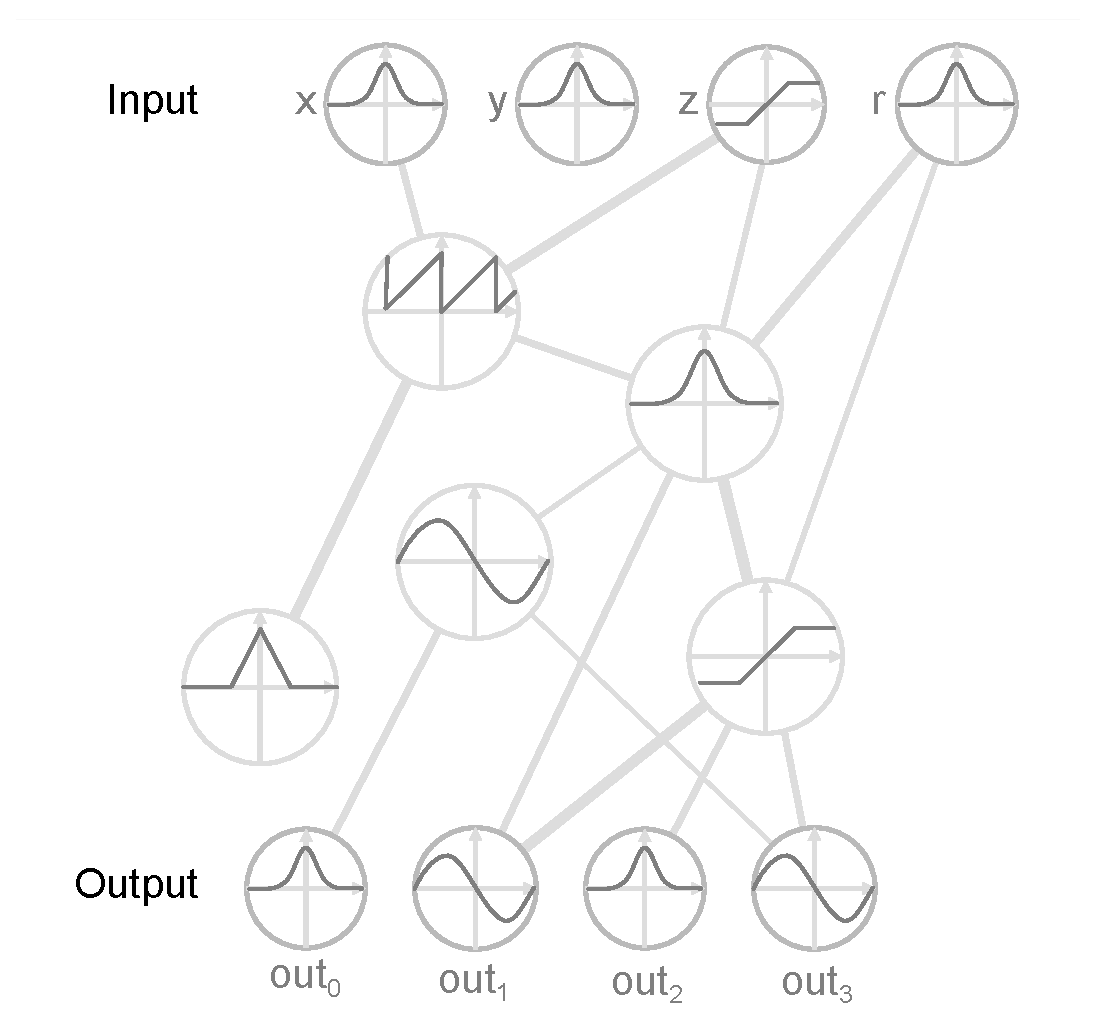
\includegraphics[width=\textwidth]{figure/CPPN}
  \caption{Close-up of a gull} \label{fig:gull} 
\end{figure}

\subsubsection{Neuroevolution of Augmenting
Topologies}
Mutating a network structure is not trivial [ref]

\section{Definition of an organism}

\subsection{Genome}

\subsection{Nervous system} \label{subsec:nervousSystem}